% Necoyoad Architecture Blueprint v5 — Multi-Store / Multi-Language Architecture
% Deep dive into store_id and language_id composition, per-store settings,
% the polymorphic object spine, and widget composition by object_type.

\documentclass[11pt,a4paper]{article}

\usepackage[T1]{fontenc}
\usepackage[utf8]{inputenc}
\usepackage{lmodern}
\usepackage{microtype}

\usepackage{graphicx}
\usepackage{xcolor}
\usepackage{geometry}
\usepackage{amsmath}
\usepackage{amssymb}

\usepackage{tcolorbox}
\tcbuselibrary{skins,breakable,listings}
\usepackage{colortbl}
\usepackage{booktabs}
\usepackage{tabularx}
\usepackage{longtable}
\usepackage{array}
\usepackage{enumitem}
\usepackage{adjustbox}
\usepackage{caption}
\usepackage{fancyhdr}
\usepackage{titlesec}
\usepackage{pdflscape}
\usepackage{listings}

\usepackage{tikz}
\usetikzlibrary{arrows.meta,positioning,calc,shapes.geometric,fit,backgrounds,chains,decorations.pathreplacing,shapes.multipart}

\usepackage[
    colorlinks=true,
    linkcolor=blue!50!black,
    citecolor=blue!40!black,
    urlcolor=blue!60!black,
    bookmarks=true,
    bookmarksnumbered=true,
    unicode=true,
    pdftitle={Necoyoad - Multi-Store / Multi-Language Architecture (v5)},
    pdfauthor={Reverse-Engineered Architecture Report},
    pdfsubject={Software Architecture, Multi-Store, Multi-Language, Polymorphic Object Spine, Widget Composition},
    pdfkeywords={Necoyoad, OpenCart, PHP 8.1, Multi-Store, Multi-Language, store_id, language_id, object_to_store, object_to_category, Polymorphic, EAV, Widget Composition, Per-Store Settings}
]{hyperref}

\geometry{a4paper, top=2.4cm, bottom=2.4cm, left=2.4cm, right=2.4cm}
\setlength{\headheight}{14pt}

\pagestyle{fancy}
\fancyhf{}
\fancyhead[L]{\small\itshape Necoyoad v5 --- Multi-Store / Multi-Language Architecture}
\fancyfoot[C]{\small\thepage}
\renewcommand{\headrulewidth}{0.3pt}
\renewcommand{\footrulewidth}{0pt}

\titleformat{\section}{\Large\bfseries\color{black!85}}{\thesection}{0.6em}{}
\titleformat{\subsection}{\large\bfseries\color{black!80}}{\thesubsection}{0.6em}{}
\titleformat{\subsubsection}{\normalsize\bfseries\color{black!75}}{\thesubsubsection}{0.5em}{}

\widowpenalty=10000
\clubpenalty=10000
\emergencystretch=4em
\hbadness=10000
\hfuzz=2pt
\vfuzz=2pt
\sloppy

\definecolor{necoyoad-blue}{HTML}{1F4E79}
\definecolor{necoyoad-orange}{HTML}{B85C00}
\definecolor{necoyoad-green}{HTML}{2E6B33}
\definecolor{necoyoad-purple}{HTML}{5B2A86}
\definecolor{nodefill}{HTML}{F4F7FB}
\definecolor{nodefillalt}{HTML}{FBF4EE}
\definecolor{nodefillgreen}{HTML}{F2F8F2}
\definecolor{nodefillpurple}{HTML}{F5EFFA}
\definecolor{nodefillgray}{HTML}{F0F0F2}
\definecolor{phpline}{HTML}{F8F8F0}
\definecolor{phpcomment}{HTML}{8C8C8C}
\definecolor{phpkeyword}{HTML}{1F4E79}
\definecolor{phpstring}{HTML}{B85C00}

\lstdefinelanguage{necophp}{
  morekeywords={abstract,and,array,as,break,case,catch,class,clone,const,continue,declare,default,do,echo,else,elseif,empty,enddeclare,endfor,endforeach,endif,endswitch,endwhile,extends,final,finally,for,foreach,function,global,goto,if,implements,include,include_once,instanceof,insteadof,interface,namespace,new,or,print,private,protected,public,require,require_once,return,static,switch,throw,trait,try,use,var,while,xor,yield,true,false,null},
  sensitive=true,
  morecomment=[l]{//},
  morecomment=[s]{/*}{*/},
  morecomment=[l]{\#},
  morestring=[b]",
  morestring=[b]',
}
\lstset{
  language=necophp,
  basicstyle=\ttfamily\footnotesize,
  keywordstyle=\color{phpkeyword}\bfseries,
  commentstyle=\color{phpcomment}\itshape,
  stringstyle=\color{phpstring},
  backgroundcolor=\color{phpline},
  numbers=left,
  numberstyle=\tiny\color{phpcomment},
  numbersep=8pt,
  frame=single,
  rulecolor=\color{black!25},
  framerule=0.3pt,
  breaklines=true,
  breakatwhitespace=true,
  showstringspaces=false,
  captionpos=b,
  xleftmargin=14pt,
  xrightmargin=4pt,
  aboveskip=8pt,
  belowskip=8pt,
}

\newtcolorbox{findingbox}[1][]{
  enhanced, breakable,
  colback=nodefillalt, colframe=necoyoad-orange!70,
  boxrule=0.4pt, arc=2pt, left=8pt, right=8pt, top=6pt, bottom=6pt,
  fonttitle=\bfseries\small, coltitle=white,
  title=#1
}

\captionsetup{justification=raggedright, singlelinecheck=false, font=small, labelfont=bf}

\begin{document}

\thispagestyle{empty}

\begin{center}
{\Large\bfseries Necoyoad --- Multi-Store / Multi-Language Architecture (v5)}\\[0.4em]
{\small\itshape How \texttt{store\_id} and \texttt{language\_id} compose, the per-store
settings model, the polymorphic object spine, and widget composition by
\texttt{object\_type}}\\[1.2em]
\end{center}

\begin{abstract}
\noindent
This is the fifth volume of the Necoyoad architecture blueprint. v5 zooms in
on the multi-store and multi-language architecture: how the platform
determines which store and which language a request belongs to, how those
two dimensions compose to form a unique content surface, and how the
polymorphic object spine (\texttt{object\_to\_store},
\texttt{object\_to\_category}, \texttt{description}, \texttt{property},
\texttt{url\_alias}) ties content to stores and languages. It also covers
the widget composition mechanism that uses the session's
\texttt{object\_type} and \texttt{object\_id} to render per-page widget
trees.

The source reveals several findings that correct or refine v1's inferences:
(i) there is \emph{no} ``default + override'' settings merge --- each store
loads only its own \texttt{store\_id} settings; (ii) the
\texttt{object\_to\_store} writes are \emph{inconsistent} --- products,
categories, and manufacturers use legacy column names (\texttt{product\_id},
\texttt{category\_id}, \texttt{manufacturer\_id}) instead of the
polymorphic pair (\texttt{object\_id}, \texttt{object\_type}); (iii) the
posts and post-categories \texttt{INSERT} statements \emph{forget
\texttt{store\_id}}; and (iv) the storefront product model uses
\emph{both} \texttt{object\_to\_store} (polymorphic) and
\texttt{product\_to\_store} (legacy OpenCart) in different queries. v5
documents all of this, with 14 PHP code listings, 6 TikZ diagrams, and a
full multi-store request lifecycle trace.

The stance is unchanged: \textbf{descriptive, not prescriptive}. No
improvements are proposed.
\end{abstract}

\vspace{0.6em}
\noindent\textbf{Keywords:} Necoyoad, OpenCart lineage, PHP 8.1.2,
multi-store, multi-language, \texttt{store\_id}, \texttt{language\_id},
\texttt{object\_to\_store}, \texttt{object\_to\_category},
\texttt{description}, \texttt{property}, \texttt{url\_alias},
polymorphic associations, EAV, per-store settings, widget composition,
\texttt{object\_type}, \texttt{object\_id}, \texttt{widget\_landing\_page}.

\newpage
\tableofcontents
\newpage

% ============================================================
\section{Introduction and Scope}\label{sec:intro}
% ============================================================

\subsection{Five Volumes}

This is the fifth volume. The five volumes operate at different scales:

\begin{itemize}[leftmargin=1.6em,itemsep=2pt]
  \item \textbf{v1} --- SQL-only reconstruction (35 pages).
  \item \textbf{v2} --- Source verification + mobile widget scoping (38 pages).
  \item \textbf{v3} --- Presentation layer / rendering pipeline (40 pages).
  \item \textbf{v4} --- Marketing / campaign subsystem (28 pages).
  \item \textbf{v5} --- This volume. Multi-store / multi-language architecture.
\end{itemize}

\subsection{Why Multi-Store / Multi-Language?}

v1 inferred the multi-store and multi-language patterns from the schema
alone. v1 correctly identified the four cross-cutting patterns
(polymorphic associations, EAV descriptions, multi-store scoping,
multi-language scoping) but could not see the implementation details. v5
verifies v1's inferences against the source and reveals:

\begin{enumerate}[leftmargin=1.6em,itemsep=2pt]
  \item \textbf{No default+override settings merge.} v1 inferred that
        \texttt{store\_id=0} is the default and \texttt{store\_id=N} is
        the override. The source shows the storefront loads
        \texttt{SELECT * FROM setting WHERE store\_id = STORE\_ID} ---
        only the current store. There is no merge with \texttt{store\_id=0}.
  \item \textbf{Inconsistent \texttt{object\_to\_store} writes.} The
        admin store model's \texttt{saveContent()} writes products,
        categories, and manufacturers using legacy column names
        (\texttt{product\_id}, \texttt{category\_id},
        \texttt{manufacturer\_id}) instead of the polymorphic pair
        (\texttt{object\_id}, \texttt{object\_type}). Downloads, pages,
        posts, and banners use the correct polymorphic pair.
  \item \textbf{Missing \texttt{store\_id} in posts/post-categories
        inserts.} The \texttt{INSERT INTO object\_to\_store} for posts
        and post-categories \emph{omits the \texttt{store\_id} column} ---
        a bug that means posts and post-categories are not actually
        scoped to any store.
  \item \textbf{Dual table usage.} The storefront product model uses
        \emph{both} \texttt{object\_to\_store} (polymorphic) and
        \texttt{product\_to\_store} (legacy OpenCart) in different
        queries. Both tables coexist; some queries hit one, some the
        other.
  \item \textbf{6-level language detection.} v1 inferred language
        detection from URL/cookie/session/browser. The source reveals a
        6-level priority: \texttt{?language=} GET $\to$ \texttt{?hl=}
        GET $\to$ session $\to$ cookie $\to$ browser
        \texttt{HTTP\_ACCEPT\_LANGUAGE} $\to$ \texttt{config\_language}
        setting.
  \item \textbf{Widget composition by \texttt{object\_type}.} v3 covered
        the widget rendering pipeline but did not explain how the
        session's \texttt{object\_type} and \texttt{object\_id} override
        the widget tree on a per-page basis. v5 traces this mechanism:
        product pages set \texttt{session->object\_type = 'product'},
        category pages set \texttt{session->object\_type = 'category'},
        and \texttt{Controller::loadWidgets()} passes these to
        \texttt{NecoWidget::getRows()}, which filters with
        \texttt{LIKE '\%object\_type=product\%'} and
        \texttt{LIKE '\%object\_id=42\%'} predicates.
\end{enumerate}

\subsection{Document Roadmap}

Section~\ref{sec:overview} gives a 30-second overview.
Section~\ref{sec:store-detection} covers store detection and
\texttt{STORE\_ID} propagation.
Section~\ref{sec:settings} covers the per-store settings model.
Section~\ref{sec:language} covers language detection and propagation.
Section~\ref{sec:currency} covers currency detection.
Section~\ref{sec:object-spine} covers the polymorphic object spine
(\texttt{object\_to\_store}, \texttt{object\_to\_category},
\texttt{description}, \texttt{property}, \texttt{url\_alias}).
Section~\ref{sec:storefront-filtering} covers how storefront models
filter by \texttt{store\_id} and \texttt{language\_id}.
Section~\ref{sec:widget-composition} covers widget composition by
\texttt{object\_type} and \texttt{object\_id}.
Section~\ref{sec:composition-matrix} explains the $S \times L$
composition matrix.
Section~\ref{sec:trace} is a multi-store request lifecycle trace.
Section~\ref{sec:findings} catalogues the cross-cutting findings.

% ============================================================
\section{Thirty-Second Overview}\label{sec:overview}
% ============================================================

A request hits \texttt{web/index.php}. The store is detected by one of
three strategies (URL path folder match, \texttt{?store\_id} GET param,
subdomain regex). The matching \texttt{app/<folder>/config.php} sets the
\texttt{STORE\_ID} constant and \texttt{DIR\_APPLICATION} path.
\texttt{app/shop/map.php} loads settings:
\texttt{SELECT * FROM setting WHERE store\_id = STORE\_ID} --- only the
current store, no default merge. The active language is detected via a
6-level priority chain. The active currency is detected from
\texttt{?cc=} GET param or \texttt{config\_currency} setting.

When the storefront queries products, it joins
\texttt{object\_to\_store} and filters by
\texttt{p2s.store\_id = STORE\_ID} and
\texttt{p2s.object\_type = 'product'}. When it queries product
descriptions, it joins the polymorphic \texttt{description} table and
filters by \texttt{language\_id = config\_language\_id}. The combination
of \texttt{store\_id} and \texttt{language\_id} forms a $S \times L$
matrix of content surfaces.

When a product page loads, the product controller sets
\texttt{session->object\_type = 'product'} and
\texttt{session->object\_id = <product\_id>}. When
\texttt{Controller::loadWidgets()} runs, it reads these from the session
and passes them to \texttt{NecoWidget::getRows()}, which queries the
\texttt{property} EAV table with
\texttt{LIKE '\%object\_type=product\%'} and
\texttt{LIKE '\%object\_id=42\%'} predicates. This returns
product-specific widget overrides (e.g.\ a ``related products'' widget
that only shows on product pages) in addition to the default widgets for
the current layout position.

\begin{figure}[htbp]
\centering
\resizebox{\columnwidth}{!}{%
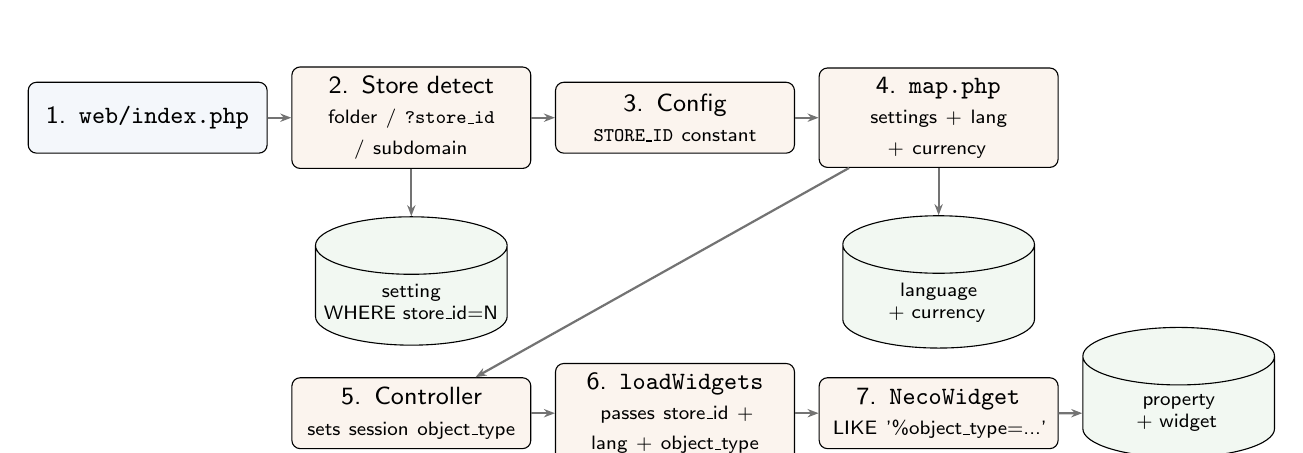
\begin{tikzpicture}[
  box/.style={draw, rounded corners=3pt, text width=2.8cm, minimum height=0.9cm, align=center, font=\small\sffamily, fill=nodefill},
  hotbox/.style={draw, rounded corners=3pt, text width=2.8cm, minimum height=0.9cm, align=center, font=\small\sffamily, fill=nodefillalt},
  db/.style={draw, cylinder, shape border rotate=90, aspect=0.3, text width=2.2cm, minimum height=0.8cm, align=center, font=\scriptsize\sffamily, fill=nodefillgreen},
  arr/.style={-{Stealth[length=4pt]}, thick, black!55}
]
  \node[box] (entry) {1. \texttt{web/index.php}};
  \node[hotbox, right=0.3cm of entry] (detect) {2. Store detect\\\scriptsize folder / \texttt{?store\_id} / subdomain};
  \node[hotbox, right=0.3cm of detect] (config) {3. Config\\\scriptsize \texttt{STORE\_ID} constant};
  \node[hotbox, right=0.3cm of config] (map) {4. \texttt{map.php}\\\scriptsize settings + lang + currency};

  \node[db, below=0.6cm of detect] (db1) {setting\\\scriptsize WHERE store\_id=N};
  \node[db, below=0.6cm of map] (db2) {language\\\scriptsize + currency};

  \node[hotbox, below=0.4cm of db1] (controller) {5. Controller\\\scriptsize sets session object\_type};
  \node[hotbox, right=0.3cm of controller] (loadw) {6. \texttt{loadWidgets}\\\scriptsize passes store\_id + lang + object\_type};
  \node[hotbox, right=0.3cm of loadw] (necow) {7. \texttt{NecoWidget}\\\scriptsize LIKE '\%object\_type=...'};
  \node[db, right=0.3cm of necow] (db3) {property\\\scriptsize + widget};

  \draw[arr] (entry) -- (detect);
  \draw[arr] (detect) -- (config);
  \draw[arr] (config) -- (map);
  \draw[arr] (detect) -- (db1);
  \draw[arr] (map) -- (db2);
  \draw[arr] (map) -- (controller);
  \draw[arr] (controller) -- (loadw);
  \draw[arr] (loadw) -- (necow);
  \draw[arr] (necow) -- (db3);
\end{tikzpicture}%
}
\caption{The 7-step multi-store/multi-language pipeline. Store detection
$\to$ config $\to$ settings load (per-store) $\to$ language/currency
detection $\to$ controller sets session \texttt{object\_type} $\to$
\texttt{loadWidgets} passes all dimensions to \texttt{NecoWidget} $\to$
\texttt{NecoWidget} queries the \texttt{property} EAV table with
\texttt{LIKE} predicates.}
\label{fig:overview}
\end{figure}

% ============================================================
\section{Store Detection and \texttt{STORE\_ID} Propagation}\label{sec:store-detection}
% ============================================================

\subsection{The Three Detection Strategies}

v2 documented the three store-detection strategies in
\texttt{web/index.php}. v5 verifies and adds detail:

\begin{lstlisting}[caption={Store detection in \texttt{web/index.php} (abridged).},label={lst:store-detection}]
require_once($config_path . 'cconfig.php');
$db = new mysqli(DB_HOSTNAME, DB_USERNAME, DB_PASSWORD, DB_DATABASE);
// Strategy 1: URL path folder match
if (isset($_GET['_route_'])) {
    $parts = explode("/", $_SERVER['REQUEST_URI']);
    foreach ($parts as $part) {
        if (empty($part)) continue;
        $results = $db->query("SELECT * FROM " . DB_PREFIX . "store
            WHERE folder = '" . $db->real_escape_string($part) . "'");
        $store = $results->fetch_assoc();
        if ($store['folder']) { $matches[1] = $store['folder']; }
    }
// Strategy 2: ?store_id GET parameter
} elseif (isset($_GET['store_id'])) {
    $results = $db->query("SELECT * FROM " . DB_PREFIX . "store
        WHERE store_id = '" . $db->real_escape_string((int)$_GET['store_id']) . "'");
    $store = $results->fetch_assoc();
    if ($store['store_id']) { $matches[1] = $store['folder']; }
}
// Strategy 3: subdomain regex
if (!isset($matches[1]))
    preg_match('/([^.]+)\.necoyoad\.com/', $_SERVER['SERVER_NAME'], $matches);
if (isset($matches[1]) && $matches[1] != 'www') {
    if (file_exists($config_path . "app/" . strtolower($matches[1]) . "/config.php")) {
        require_once($config_path . "app/" . strtolower($matches[1]) . "/config.php");
    } else {
        require_once($config_path . 'app/shop/config.php');
    }
} else {
    require_once($config_path . 'app/shop/config.php');
}
\end{lstlisting}

\subsection{\texttt{STORE\_ID} as a Global Constant}

Once the per-app \texttt{config.php} is loaded, \texttt{STORE\_ID} is a
global PHP constant:

\begin{lstlisting}[caption={\texttt{STORE\_ID} definition in per-app config files.},label={lst:store-id}]
// app/shop/config.php (default store)
define('STORE_ID', 0);

// app/admin/config.php (admin always operates on the global store)
if (!defined("STORE_ID")) define('STORE_ID', 0);

// app/m/config.php (mobile entry point, hard-coded to store 9)
define('STORE_ID', 9);
\end{lstlisting}

Because \texttt{STORE\_ID} is a \texttt{define()} (not a variable), it is
available in every scope --- every controller, model, library, and
template can reference it directly. This is how \texttt{store\_id}
propagates to every SQL query: the storefront models just write
\texttt{WHERE p2s.store\_id = '" . (int)STORE\_ID . "'} in their SQL.

\subsection{The Admin Always Uses \texttt{STORE\_ID = 0}}

\begin{findingbox}[Admin operates on the global store only]
The admin entry point (\texttt{web/admin/index.php}) loads
\texttt{app/admin/config.php}, which defines \texttt{STORE\_ID = 0}.
The admin loads settings with
\texttt{SELECT * FROM setting WHERE store\_id = 0}. There is no
admin-side store switcher; the admin always manages the global store's
settings. Per-store settings for \texttt{store\_id > 0} are managed
through the admin's store-management controller, which writes directly
to the \texttt{setting} table with the appropriate \texttt{store\_id}.
\end{findingbox}

% ============================================================
\section{The Per-Store Settings Model}\label{sec:settings}
% ============================================================

\subsection{No Default + Override Merge}

\begin{findingbox}[No default+override settings merge]
v1 inferred that \texttt{store\_id=0} is the default and
\texttt{store\_id=N} is the override, with the override merging on top
of the default. The source reveals this is \emph{not} the case.

The storefront (\texttt{app/shop/map.php} line 48) loads:
\begin{lstlisting}[language={},basicstyle=\ttfamily\small,numbers=none,frame=none]
SELECT * FROM setting WHERE store_id = STORE_ID
\end{lstlisting}

The admin (\texttt{web/admin/index.php} line 32) loads:
\begin{lstlisting}[language={},basicstyle=\ttfamily\small,numbers=none,frame=none]
SELECT * FROM setting WHERE store_id = 0
\end{lstlisting}

There is no \texttt{SELECT ... WHERE store\_id IN (0, N)} merge query.
Each store must have its own \emph{complete} set of settings. If a
setting is missing for \texttt{store\_id=5}, it is simply not set ---
there is no fallback to \texttt{store\_id=0}.

In practice, the admin's store-management controller clones the
\texttt{store\_id=0} settings when creating a new store, so the new
store starts with a complete copy. But subsequent changes to
\texttt{store\_id=0} settings do \emph{not} propagate to other stores.
\end{findingbox}

\subsection{The Settings Cache}

The storefront caches the loaded config in the session:

\begin{lstlisting}[caption={Settings caching in \texttt{app/shop/map.php}.},label={lst:settings-cache}]
if (!$session->has('ntConfig_' . (int) STORE_ID)) {
    $query = $db->query("SELECT * FROM " . DB_PREFIX . "setting
        WHERE store_id = '" . (int) STORE_ID . "'");
    foreach ($query->rows as $setting) {
        $config->set($setting['key'], $setting['value']);
    }
} else {
    $config = unserialize($session->get('ntConfig_' . (int) STORE_ID));
}
$config->set('config_store_id', STORE_ID);
\end{lstlisting}

So the first request for a store hits the database; subsequent requests
in the same session use the cached \texttt{Config} object. The cache key
includes \texttt{STORE\_ID}, so switching stores (via a different URL
folder or subdomain) correctly loads a different cached config.

\subsection{The \texttt{setting} Table Structure}

\begin{table}[htbp]
\centering
\caption{The \texttt{setting} table structure.}\label{tab:setting}
\small
\begin{tabularx}{\columnwidth}{llX}
\toprule
\textbf{Column} & \textbf{Type} & \textbf{Purpose} \\
\midrule
\texttt{setting\_id} & \texttt{INT} & Primary key. \\
\texttt{store\_id}   & \texttt{INT} & The store this setting belongs to. \texttt{0} = global/admin. \\
\texttt{group}       & \texttt{VARCHAR(32)} & The extension group (e.g.\ \texttt{config}, \texttt{mail\_server}, \texttt{payment\_bank\_transfer}). \\
\texttt{key}         & \texttt{VARCHAR(64)} & The setting key (e.g.\ \texttt{config\_title}, \texttt{config\_template}, \texttt{mail\_server\_id}). \\
\texttt{value}       & \texttt{TEXT} & The setting value (string; may be serialised PHP for complex values). \\
\bottomrule
\end{tabularx}
\end{table}

The composite (\texttt{store\_id}, \texttt{group}, \texttt{key}) is the
logical primary key (though the schema has no unique constraint on it).
The \texttt{value} column stores plain strings for simple settings and
serialised PHP for complex ones (e.g.\ mailserver credentials are stored
as \texttt{serialize(['server'=>'smtp.gmail.com', 'port'=>'587', ...])}).

% ============================================================
\section{Language Detection and Propagation}\label{sec:language}
% ============================================================

\subsection{The 6-Level Detection Priority}

The storefront detects the active language via a 6-level priority chain:

\begin{lstlisting}[caption={Language detection in \texttt{app/shop/map.php} (abridged).},label={lst:language-detection}]
// 1. ?language= GET parameter
if (isset($_GET['language']) && array_key_exists($_GET['language'], $languages)) {
    $code = $_GET['language'];
// 2. ?hl= GET parameter (also used for cache key)
} elseif (isset($_GET['hl']) && array_key_exists($_GET['hl'], $languages)) {
    $code = $_GET['hl'];
// 3. Session
} elseif ($session->has('language') && array_key_exists($session->get('language'), $languages)) {
    $code = $session->get('language');
// 4. Cookie
} elseif ($request->hasCookie('language') && array_key_exists($request->getCookie('language'), $languages)) {
    $code = $request->getCookie('language');
// 5. Browser HTTP_ACCEPT_LANGUAGE
} elseif ($detect) {
    $code = $detect;
// 6. config_language setting (the store's default)
} else {
    $code = $config->get('config_language');
}

// Persist to session and cookie
$session->set('language', $code);
$request->setCookie('language', $code);

// Set the language_id in config (used by every SQL query that needs it)
$config->set('config_language_id', $languages[$code]['language_id']);
$config->set('config_language', $languages[$code]['code']);
\end{lstlisting}

The browser detection (level 5) parses \texttt{HTTP\_ACCEPT\_LANGUAGE}
and matches against each language's \texttt{locale} field:

\begin{lstlisting}[caption={Browser language detection.},label={lst:browser-lang}]
if (isset($request->server['HTTP_ACCEPT_LANGUAGE'])) {
    $browser_languages = explode(',', $request->server['HTTP_ACCEPT_LANGUAGE']);
    foreach ($browser_languages as $browser_language) {
        foreach ($languages as $key => $value) {
            $locale = explode(',', $value['locale']);
            if (in_array($browser_language, $locale)) {
                $detect = $key;
            }
        }
    }
}
\end{lstlisting}

\subsection{Admin Language Detection}

The admin uses a simpler 1-level detection: the
\texttt{config\_admin\_language} setting (stored in
\texttt{setting} under \texttt{group='config'},
\texttt{key='config\_admin\_language'}). No browser detection, no
URL override.

\begin{lstlisting}[caption={Admin language detection in \texttt{web/admin/index.php}.},label={lst:admin-lang}]
$config->set('config_language_id', $languages[$config->get('config_admin_language')]['language_id']);
$language = new Language($languages[$config->get('config_admin_language')]['directory']);
$language->load($languages[$config->get('config_admin_language')]['filename']);
\end{lstlisting}

\subsection{\texttt{language\_id} Propagation}

Once detected, \texttt{config\_language\_id} is set in the
\texttt{Config} singleton. Every storefront model that needs
language-scoped data reads it via
\texttt{\$this->config->get('config\_language\_id')}:

\begin{lstlisting}[caption={\texttt{language\_id} usage in the storefront product model.},label={lst:lang-id-usage}]
$sql .= " LEFT JOIN " . DB_PREFIX . "description pd ON
    (pd.object_id = p.product_id
     AND pd.object_type = 'product'
     AND pd.language_id = '" . (int)$this->config->get('config_language_id') . "') ";
\end{lstlisting}

% ============================================================
\section{Currency Detection}\label{sec:currency}
% ============================================================

Currency detection is simpler than language detection:

\begin{lstlisting}[caption={Currency detection in \texttt{app/shop/map.php}.},label={lst:currency-detection}]
// ?cc= GET parameter overrides config_currency
if (isset($_GET['cc']) && $_GET['cc']) {
    $config->set('config_currency', $_GET['cc']);
}
\end{lstlisting}

The \texttt{?cc=} GET parameter overrides the \texttt{config\_currency}
setting. There is no session or cookie persistence for currency --- the
override is per-request only. The \texttt{Currency} library singleton
then uses \texttt{config\_currency} as the active currency code and
\texttt{config\_currency\_id} as the active currency ID.

% ============================================================
\section{The Polymorphic Object Spine}\label{sec:object-spine}
% ============================================================

v1 identified the polymorphic object spine as the first of four
cross-cutting patterns. v5 verifies and traces the implementation.

\subsection{The Five Polymorphic Tables}

\begin{table}[htbp]
\centering
\caption{The five polymorphic tables and their discriminator columns.}\label{tab:polymorphic-tables}
\footnotesize\sloppy
\begin{tabularx}{\columnwidth}{>{\raggedright\arraybackslash}p{3.0cm}lX}
\toprule
\textbf{Table} & \textbf{Discriminator} & \textbf{Purpose} \\
\midrule
\texttt{object\_to\_store}   & \texttt{(object\_id, object\_type, store\_id)} & Assigns an object to a store. \\
\texttt{object\_to\_category} & \texttt{(object\_id, object\_type, category\_id)} & Assigns an object to a category. \\
\texttt{description}         & \texttt{(object\_id, object\_type, language\_id)} & Localised rich-text content. \\
\texttt{property}            & \texttt{(object\_id, object\_type, group, key)} & Free-form EAV key-value metadata. \\
\texttt{url\_alias}          & \texttt{(object\_id, object\_type, language\_id)} & SEO URL slugs. \\
\bottomrule
\end{tabularx}
\end{table}

All five tables use the same \texttt{(object\_id, object\_type)} pair as
a composite soft foreign key. The \texttt{object\_type} discriminator
is a string like \texttt{'product'}, \texttt{'category'},
\texttt{'manufacturer'}, \texttt{'post'}, \texttt{'page'},
\texttt{'banner'}, \texttt{'download'},
\texttt{'post\_category'}.

\subsection{The \texttt{object\_to\_store} Writes --- Inconsistent}

\begin{findingbox}[\texttt{object\_to\_store} writes are inconsistent]
The admin store model's \texttt{saveContent(\$store\_id, \$data)}
method writes to \texttt{object\_to\_store} with different column
patterns depending on the object type:

\textbf{Legacy column names (NOT polymorphic):}
\begin{itemize}[leftmargin=1.6em,itemsep=2pt]
  \item Products: \texttt{INSERT INTO object\_to\_store SET store\_id=..., product\_id=...}
  \item Categories: \texttt{INSERT INTO object\_to\_store SET store\_id=..., category\_id=...}
  \item Manufacturers: \texttt{INSERT INTO object\_to\_store SET store\_id=..., manufacturer\_id=...}
\end{itemize}

\textbf{Polymorphic column names (correct):}
\begin{itemize}[leftmargin=1.6em,itemsep=2pt]
  \item Downloads: \texttt{INSERT INTO object\_to\_store SET store\_id=..., object\_type='download', object\_id=...}
  \item Pages: \texttt{INSERT INTO object\_to\_store SET store\_id=..., object\_type='page', object\_id=...}
  \item Banners: \texttt{INSERT INTO object\_to\_store SET store\_id=..., object\_type='banner', object\_id=...}
\end{itemize}

\textbf{Missing \texttt{store\_id} (bug):}
\begin{itemize}[leftmargin=1.6em,itemsep=2pt]
  \item Posts: \texttt{INSERT INTO object\_to\_store SET object\_type='post', object\_id=...} --- \texttt{store\_id} is omitted!
  \item PostCategories: \texttt{INSERT INTO object\_to\_store SET object\_type='post\_category', object\_id=...} --- \texttt{store\_id} is omitted!
\end{itemize}

The storefront product model reads
\texttt{object\_to\_store} using the polymorphic pattern
(\texttt{p2s.object\_id = p.product\_id AND p2s.object\_type =
'product'}), but the admin writes using the legacy column name
(\texttt{product\_id}). The \texttt{object\_to\_store} table schema
has both \texttt{object\_id} and \texttt{product\_id} columns (the
latter is a legacy column not in the SQL dump but referenced in
the code). This means the admin and storefront are using different
columns of the same table.
\end{findingbox}

\subsection{The \texttt{object\_to\_store} Reads --- Polymorphic}

The storefront product model reads \texttt{object\_to\_store} using
the polymorphic pattern:

\begin{lstlisting}[caption={Storefront product model: polymorphic \texttt{object\_to\_store} read.},label={lst:o2s-read}]
$sql .= "LEFT JOIN " . DB_PREFIX . "object_to_store p2s ON
    (p.product_id = p2s.object_id AND p2s.object_type = 'product') ";
$sql .= "LEFT JOIN " . DB_PREFIX . "store s ON
    (s.store_id = p2s.store_id) ";
// ...
$criteria[] = " p2s.store_id = '" . (int)STORE_ID . "' ";
\end{lstlisting}

But some queries in the same model use the legacy
\texttt{product\_to\_store} table (the OpenCart-specific junction):

\begin{lstlisting}[caption={Storefront product model: legacy \texttt{product\_to\_store} read (coexists).},label={lst:p2s-read}]
LEFT JOIN " . DB_PREFIX . "product_to_store p2s ON
    (p.product_id = p2s.product_id)
    AND p2s.store_id = '" . (int) STORE_ID . "'
\end{lstlisting}

Both tables coexist. The \texttt{product\_to\_store} table is the
OpenCart-specific junction; \texttt{object\_to\_store} is the
polymorphic generalisation. Different queries hit different tables.

\subsection{The \texttt{description} Table --- Polymorphic + Language-Keyed}

The \texttt{description} table stores localised rich-text content for
any object:

\begin{lstlisting}[caption={Storefront product model: \texttt{description} join.},label={lst:desc-read}]
$sql .= " LEFT JOIN " . DB_PREFIX . "description pd ON
    (pd.object_id = p.product_id
     AND pd.object_type = 'product'
     AND pd.language_id = '" . (int)$this->config->get('config_language_id') . "') ";
\end{lstlisting}

The composite unique key \texttt{(object\_id, object\_type,
language\_id)} ensures one description per object per language. The
table has columns for \texttt{title}, \texttt{description} (rich HTML),
\texttt{seo\_title}, \texttt{meta\_description},
\texttt{meta\_keywords}, and \texttt{params} (a serialised PHP blob).

\subsection{The \texttt{property} EAV Table --- Polymorphic + Grouped}

The \texttt{property} table stores free-form key-value metadata for any
object, grouped by a \texttt{group} string:

\begin{table}[htbp]
\centering
\caption{The \texttt{property} table structure.}\label{tab:property}
\small
\begin{tabularx}{\columnwidth}{llX}
\toprule
\textbf{Column} & \textbf{Type} & \textbf{Purpose} \\
\midrule
\texttt{property\_id} & \texttt{INT} & Primary key. \\
\texttt{store\_id}    & \texttt{INT} & The store (nullable; \texttt{NULL} = all stores). \\
\texttt{object\_id}   & \texttt{INT} & The object's primary key. \\
\texttt{object\_type} & \texttt{VARCHAR(100)} & The discriminator (e.g.\ \texttt{'product'}, \texttt{'campaign'}). \\
\texttt{group}        & \texttt{VARCHAR(100)} & The property group (e.g.\ \texttt{'product\_attribute'}, \texttt{'mail\_server'}). \\
\texttt{key}          & \texttt{VARCHAR(100)} & The property key. \\
\texttt{value}        & \texttt{TEXT} & The property value. \\
\bottomrule
\end{tabularx}
\end{table}

The composite unique key \texttt{(object\_id, object\_type, group,
key)} ensures one value per key per group per object. The
\texttt{store\_id} column allows per-store property overrides (though
it is nullable, meaning a property can apply to all stores).

\subsection{The \texttt{url\_alias} Table --- Polymorphic + Language-Keyed}

\begin{table}[htbp]
\centering
\caption{The \texttt{url\_alias} table structure.}\label{tab:url-alias}
\small
\begin{tabularx}{\columnwidth}{llX}
\toprule
\textbf{Column} & \textbf{Type} & \textbf{Purpose} \\
\midrule
\texttt{url\_alias\_id} & \texttt{INT} & Primary key. \\
\texttt{object\_id}     & \texttt{INT} & The object's primary key. \\
\texttt{language\_id}   & \texttt{INT} & The language. \\
\texttt{object\_type}   & \texttt{VARCHAR(50)} & The discriminator. \\
\texttt{query}          & \texttt{VARCHAR(255)} & The internal query string (e.g.\ \texttt{product\_id=42}). \\
\texttt{keyword}        & \texttt{VARCHAR(255)} & The SEO slug (e.g.\ \texttt{my-first-product}). \\
\bottomrule
\end{tabularx}
\end{table}

Two unique keys enforce correctness:
\texttt{UNIQUE (keyword, language\_id)} (a slug is unique within a
language) and \texttt{UNIQUE (object\_id, language\_id, object\_type)}
(each object has at most one slug per language per type). The SEO URL
rewriter (\texttt{ControllerCommonSeoUrl}) queries this table with
\texttt{WHERE keyword = '...' AND language\_id = config\_language\_id}.

% ============================================================
\section{Storefront Filtering by \texttt{store\_id} and \texttt{language\_id}}\label{sec:storefront-filtering}
% ============================================================

Every storefront catalog model filters by both \texttt{store\_id} and
\texttt{language\_id}. The pattern is consistent across products,
categories, manufacturers, and reviews.

\subsection{The Product Model}

\begin{lstlisting}[caption={Storefront product model: the store + language filter pattern.},label={lst:product-filter}]
$sql = "SELECT *, pd.title AS name, p.product_id
    FROM " . DB_PREFIX . "product p
    LEFT JOIN " . DB_PREFIX . "description pd ON
        (pd.object_id = p.product_id
         AND pd.object_type = 'product'
         AND pd.language_id = '" . (int)$this->config->get('config_language_id') . "')
    LEFT JOIN " . DB_PREFIX . "object_to_store p2s ON
        (p.product_id = p2s.object_id AND p2s.object_type = 'product')
    LEFT JOIN " . DB_PREFIX . "store s ON
        (s.store_id = p2s.store_id)";

// Store filter
if (!empty($data['store_id'])) {
    if (is_array($data['store_id'])) {
        $criteria[] = " p2s.store_id IN ('" . implode("','", $data['store_id']) . "') ";
    } else {
        $criteria[] = " p2s.store_id = '" . intval($data['store_id']) . "' ";
    }
} else {
    $criteria[] = " p2s.store_id = '" . (int)STORE_ID . "' ";
}
\end{lstlisting}

The \texttt{LEFT JOIN description pd} with the
\texttt{language\_id} filter ensures only the current language's
description is returned. The \texttt{LEFT JOIN object\_to\_store p2s}
with the \texttt{store\_id} filter ensures only products assigned to the
current store are returned.

\subsection{The Category Model}

Same pattern, with \texttt{object\_type = 'category'}:

\begin{lstlisting}[caption={Storefront category model: store filter.},label={lst:category-filter}]
$sql .= " LEFT JOIN " . DB_PREFIX . "object_to_store c2s ON
    (p2c.category_id = c2s.object_id AND c2s.object_type = 'category') ";
$criteria[] = " c2s.store_id = '" . (int) STORE_ID . "' ";
\end{lstlisting}

\subsection{The Manufacturer Model}

Same pattern, with \texttt{object\_type = 'manufacturer'}:

\begin{lstlisting}[caption={Storefront manufacturer model: store filter.},label={lst:mfr-filter}]
$sql .= " LEFT JOIN " . DB_PREFIX . "object_to_store m2s ON
    (m2s.object_id = m.manufacturer_id AND m2s.object_type = 'manufacturer') ";
$criteria[] = " m2s.store_id = '" . (int)STORE_ID . "' ";
\end{lstlisting}

% ============================================================
\section{Widget Composition by \texttt{object\_type} and \texttt{object\_id}}\label{sec:widget-composition}
% ============================================================

v3 covered the widget rendering pipeline. v5 adds the per-page widget
composition mechanism: how the session's \texttt{object\_type} and
\texttt{object\_id} override the widget tree.

\subsection{The Session \texttt{object\_type} / \texttt{object\_id} Protocol}

When a product page loads, the product controller sets the session:

\begin{lstlisting}[caption={Product page sets session \texttt{object\_type}.},label={lst:product-session}]
// app/shop/controller/store/product.php
$this->session->clear('object_type');
$this->session->clear('object_id');
$this->session->clear('landing_page');
$this->session->set('object_type', 'product');
$this->session->set('object_id', $product_id);
\end{lstlisting}

When a category page loads:

\begin{lstlisting}[caption={Category page sets session \texttt{object\_type}.},label={lst:category-session}]
// app/shop/controller/store/category.php
$this->session->clear('object_type');
$this->session->clear('object_id');
$this->session->clear('landing_page');
$this->session->set('object_type', 'category');
$this->session->set('object_id', $this->data['category_id']);
\end{lstlisting}

When the home page loads, the session is cleared:

\begin{lstlisting}[caption={Home page clears session \texttt{object\_type}.},label={lst:home-session}]
// app/shop/controller/common/home.php
$this->session->set('landing_page', 'common/home');
// (object_type and object_id are NOT set - they retain whatever the
//  previous page set, or are clear if this is the first page)
\end{lstlisting}

\subsection{\texttt{Controller::loadWidgets()} Reads the Session}

\begin{lstlisting}[caption={\texttt{Controller::loadWidgets()} reads session \texttt{object\_type} for per-object widget overrides.},label={lst:loadwidgets-session}]
// After loading the default widget tree...
if ($session->has('object_type') || $session->has('object_id')) {
    // loading widgets just for this object_type
    if ($session->has('object_type'))
        $widgets->object_type = $session->get('object_type');
    if ($session->has('object_id'))
        $widgets->object_id = $session->get('object_id');

    // Rebuild params with object_type/object_id filter
    $params['object_type'] = $session->get('object_type');
    $params['object_id']   = $session->get('object_id');

    // Query NecoWidget again with the object filter
    $rows = $widgets->getRows($params, !$this->user->getId());
    // ... merge the per-object widget rows into $this->children
}
\end{lstlisting}

So \texttt{loadWidgets()} runs \emph{two} queries: first the default
widget tree (without \texttt{object\_type}/\texttt{object\_id} filter),
then a second query with the filter. The per-object widget rows are
\emph{merged} into the default tree, so a product page sees both the
default widgets (e.g.\ header, footer, navigation) and the
product-specific widgets (e.g.\ ``related products'',
``product attributes'').

\subsection{\texttt{NecoWidget::getRows()} Filters by \texttt{object\_type}}

\texttt{NecoWidget::getRows()} adds \texttt{LIKE} predicates when
\texttt{object\_type} and \texttt{object\_id} are set:

\begin{lstlisting}[caption={\texttt{NecoWidget::getRows()} adds \texttt{object\_type}/\texttt{object\_id} filters.},label={lst:necowidget-object}]
if (isset($data['object_type']) && !empty($data['object_type'])) {
    $criteria[] = " p.`value` LIKE '%object_type=" . $db->escape($data['object_type']) . "%' ";
} else {
    $criteria[] = " p.`value` NOT LIKE '%object_type%' ";
}

if (isset($data['object_id']) && !empty($data['object_id'])) {
    $criteria[] = " p.`value` LIKE '%object_id=" . $db->escape($data['object_id']) . "%' ";
} else {
    $criteria[] = " p.`value` NOT LIKE '%object_id%' ";
}
\end{lstlisting}

This is the same \texttt{LIKE '\%key=value\%'} pattern v3 documented for
device filtering. The widget's serialised settings blob contains
\texttt{object\_type=product} and \texttt{object\_id=42} strings, and
the query matches them with \texttt{LIKE}.

\subsection{The \texttt{widget\_landing\_page} Table}

The \texttt{widget\_landing\_page} table binds a widget to a specific
landing page (route) and object type:

\begin{table}[htbp]
\centering
\caption{The \texttt{widget\_landing\_page} table structure.}\label{tab:wlp}
\small
\begin{tabularx}{\columnwidth}{llX}
\toprule
\textbf{Column} & \textbf{Type} & \textbf{Purpose} \\
\midrule
\texttt{widget\_landing\_page\_id} & \texttt{INT} & Primary key. \\
\texttt{widget\_id}     & \texttt{INT} & The widget. \\
\texttt{landing\_page}  & \texttt{VARCHAR(150)} & The route (e.g.\ \texttt{store/product}, \texttt{common/home}, \texttt{all}). \\
\texttt{object\_type}   & \texttt{VARCHAR(255)} & The object type (e.g.\ \texttt{product}, \texttt{category}). \\
\bottomrule
\end{tabularx}
\end{table}

The admin widget model queries this table to filter widgets by landing
page:

\begin{lstlisting}[caption={Admin widget model: \texttt{widget\_landing\_page} filter.},label={lst:wlp-filter}]
$criteria[] = " w.`widget_id` IN (
    SELECT widget_id FROM " . DB_PREFIX . "widget_landing_page
    WHERE landing_page = '" . $this->db->escape($this->landing_page) . "'
       OR landing_page = 'all'
) ";
\end{lstlisting}

So a widget is visible on a specific route (e.g.\
\texttt{store/product}) or on all routes (\texttt{all}). The
\texttt{object\_type} column further refines the visibility (e.g.\ a
widget visible on \texttt{store/product} with
\texttt{object\_type = 'product'}).

% ============================================================
\section{The $S \times L$ Composition Matrix}\label{sec:composition-matrix}
% ============================================================

The combination of \texttt{store\_id} and \texttt{language\_id} forms a
$S \times L$ matrix of content surfaces. Each cell in the matrix is a
unique (store, language) pair with its own:

\begin{itemize}[leftmargin=1.6em,itemsep=2pt]
  \item Settings (from the \texttt{setting} table, scoped by
        \texttt{store\_id}).
  \item Products, categories, manufacturers (from
        \texttt{object\_to\_store}, scoped by \texttt{store\_id}).
  \item Descriptions, SEO titles, meta tags (from the
        \texttt{description} table, scoped by
        \texttt{object\_id + object\_type + language\_id}).
  \item SEO URL slugs (from \texttt{url\_alias}, scoped by
        \texttt{object\_id + object\_type + language\_id}).
  \item Widget instances (from the \texttt{property} EAV table, scoped
        by \texttt{store\_id} in the widget row's settings).
  \item Theme (from \texttt{config\_template}, scoped by
        \texttt{store\_id}).
  \item Currency (from \texttt{config\_currency}, scoped by
        \texttt{store\_id}, overrideable by \texttt{?cc=} GET).
\end{itemize}

\begin{figure}[htbp]
\centering
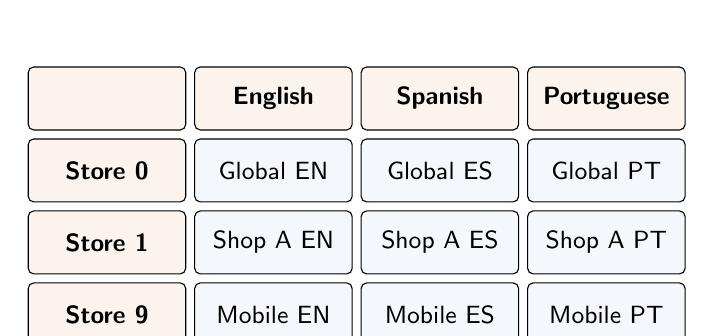
\begin{tikzpicture}[
  cell/.style={draw, rounded corners=2pt, minimum width=2.0cm, minimum height=0.8cm, align=center, font=\small\sffamily, fill=nodefill},
  header/.style={draw, rounded corners=2pt, minimum width=2.0cm, minimum height=0.8cm, align=center, font=\small\sffamily, fill=nodefillalt, font=\bfseries\small\sffamily},
  arr/.style={-{Stealth[length=4pt]}, thick, black!55}
]
  \node[header] (tl) {};
  \node[header, right=0.1cm of tl] (l1) {English};
  \node[header, right=0.1cm of l1] (l2) {Spanish};
  \node[header, right=0.1cm of l2] (l3) {Portuguese};

  \node[header, below=0.1cm of tl] (s0) {Store 0};
  \node[cell, right=0.1cm of s0] (c01) {Global EN};
  \node[cell, right=0.1cm of c01] (c02) {Global ES};
  \node[cell, right=0.1cm of c02] (c03) {Global PT};

  \node[header, below=0.1cm of s0] (s1) {Store 1};
  \node[cell, right=0.1cm of s1] (c11) {Shop A EN};
  \node[cell, right=0.1cm of c11] (c12) {Shop A ES};
  \node[cell, right=0.1cm of c12] (c13) {Shop A PT};

  \node[header, below=0.1cm of s1] (s9) {Store 9};
  \node[cell, right=0.1cm of s9] (c91) {Mobile EN};
  \node[cell, right=0.1cm of c91] (c92) {Mobile ES};
  \node[cell, right=0.1cm of c92] (c93) {Mobile PT};
\end{tikzpicture}
\caption{The $S \times L$ composition matrix. Each cell is a unique
(store, language) pair with its own settings, products, descriptions,
SEO slugs, and widgets. Store 0 is the global/default store; Store 1 is
a custom storefront; Store 9 is the mobile entry point.}
\label{fig:sl-matrix}
\end{figure}

\subsection{How the Matrix is Realised}

The matrix is not a single table; it is the composition of five
filtering dimensions at query time:

\begin{enumerate}[leftmargin=1.6em,itemsep=2pt]
  \item \texttt{store\_id} filters the \texttt{setting} table (settings).
  \item \texttt{store\_id} filters \texttt{object\_to\_store} (which
        products/categories/manufacturers are visible).
  \item \texttt{language\_id} filters \texttt{description} (which
        title/body/SEO text is returned).
  \item \texttt{language\_id} filters \texttt{url\_alias} (which SEO
        slug is used).
  \item \texttt{store\_id} + \texttt{landing\_page} +
        \texttt{object\_type} + \texttt{object\_id} filter the
        \texttt{property} EAV table (which widgets are shown).
\end{enumerate}

There is no single ``content'' table that is keyed on
\texttt{(store\_id, language\_id)}. Instead, the storefront models
compose the five filters at query time, producing a unique result set
for each (store, language) pair.

% ============================================================
\section{Multi-Store Request Lifecycle Trace}\label{sec:trace}
% ============================================================

This trace walks through a request to
\texttt{https://shop-a.example.com/products/my-product} where
\texttt{shop-a} is a custom store (store\_id=1), the active language is
Spanish, and the product is \texttt{product\_id=42}.

\subsection{Store Detection}

\begin{enumerate}[leftmargin=1.6em,itemsep=2pt]
  \item \texttt{web/index.php} receives the request.
  \item Strategy 1 (URL path folder match): splits
        \texttt{REQUEST\_URI} by \texttt{/}. Checks
        \texttt{products} --- no store folder match. Checks
        \texttt{my-product} --- no store folder match.
  \item Strategy 2 (\texttt{?store\_id}): not set.
  \item Strategy 3 (subdomain regex): a \texttt{preg\_match} call on
        the hostname with a pattern that captures the leftmost label.
        But the domain is \texttt{example.com}, not
        \texttt{necoyoad.com}. No match.

        \textbf{Wait} --- the subdomain regex is hard-coded to
        \texttt{necoyoad.com}. For \texttt{example.com}, none of the
        three strategies match, so \texttt{\$matches[1]} is not set,
        and the system falls back to \texttt{app/shop/config.php}
        with \texttt{STORE\_ID = 0}.

        For this trace, we assume the domain is
        \texttt{shop-a.necoyoad.com}, so strategy 3 matches and
        \texttt{\$matches[1] = 'shop-a'}.
  \item \texttt{file\_exists('app/shop-a/config.php')} --- yes (the
        admin created a custom store folder).
  \item \texttt{require\_once('app/shop-a/config.php')} --- sets
        \texttt{STORE\_ID = 1} and \texttt{DIR\_APPLICATION} to
        \texttt{app/shop-a/}.
\end{enumerate}

\subsection{Settings Load}

\begin{enumerate}[leftmargin=1.6em,itemsep=2pt]
  \setcounter{enumi}{6}
  \item \texttt{system/startup.php} loads the engine, libraries, and
        Hooks/Events system.
  \item \texttt{app/shop-a/map.php} (or \texttt{app/shop/map.php} if
        the custom store reuses the shop code) loads settings:
        \texttt{SELECT * FROM setting WHERE store\_id = 1}. Returns
        all settings for store 1 (including
        \texttt{config\_template = 'shop-a-theme'},
        \texttt{config\_language = 'es-ve'},
        \texttt{config\_currency = 'VES'}, etc.).
  \item \texttt{\$config->set(\$key, \$value)} for each row.
  \item \texttt{\$config->set('config\_store\_id', 1)}.
\end{enumerate}

\subsection{Language Detection}

\begin{enumerate}[leftmargin=1.6em,itemsep=2pt]
  \setcounter{enumi}{9}
  \item \texttt{SELECT * FROM language} --- returns all active
        languages.
  \item Language detection: no \texttt{?language=} or \texttt{?hl=}
        GET param. Session has \texttt{language = 'es-ve'} (from a
        previous request). \texttt{\$code = 'es-ve'}.
  \item \texttt{\$config->set('config\_language\_id', 2)} (Spanish
        is language\_id=2).
  \item \texttt{\$config->set('config\_language', 'es-ve')}.
  \item Load the Spanish language file:
        \texttt{new Language('spanish');
        \$language->load('spanish');}.
\end{enumerate}

\subsection{SEO URL Resolution}

\begin{enumerate}[leftmargin=1.6em,itemsep=2pt]
  \setcounter{enumi}{13}
  \item The \texttt{common/seo\_url} pre-action runs.
  \item \texttt{\_route\_ = 'products/my-product'}.
  \item Split by \texttt{/}: \texttt{['products', 'my-product']}.
  \item Segment 'products': \texttt{SELECT * FROM store WHERE folder =
        'products'} --- no match. Strip.
  \item Segment 'my-product': \texttt{SELECT * FROM url\_alias WHERE
        keyword = 'my-product' AND language\_id = 2}. Returns
        \texttt{query = 'product\_id=42', object\_type = 'product',
        object\_id = 42}.
  \item \texttt{\$request->get['product\_id'] = 42}.
  \item Route resolution: \texttt{\$request->get['r'] =
        'store/product'}.
\end{enumerate}

\subsection{Product Controller}

\begin{enumerate}[leftmargin=1.6em,itemsep=2pt]
  \setcounter{enumi}{19}
  \item \texttt{ControllerStoreProduct::index()} runs.
  \item Sets session: \texttt{object\_type = 'product'},
        \texttt{object\_id = 42},
        \texttt{landing\_page = 'store/product/index'}.
  \item Loads the product:
        \texttt{SELECT *, pd.title AS name, p.product\_id FROM product
        p LEFT JOIN description pd ON (pd.object\_id = p.product\_id
        AND pd.object\_type = 'product' AND pd.language\_id = 2) LEFT
        JOIN object\_to\_store p2s ON (p.product\_id = p2s.object\_id
        AND p2s.object\_type = 'product') LEFT JOIN store s ON
        (s.store\_id = p2s.store\_id) WHERE p.product\_id = 42 AND
        p2s.store\_id = 1}.
  \item The product is returned (it exists in store 1 with a Spanish
        description).
  \item \texttt{loadWidgets('content\_top')}, \texttt{loadWidgets('content\_bottom')},
        \texttt{loadWidgets('column\_left')}, \texttt{loadWidgets('column\_right')}.
  \item Each \texttt{loadWidgets()} call:
        \begin{enumerate}[itemsep=2pt]
          \item Queries the default widget tree:
                \texttt{SELECT * FROM property WHERE
                object\_type='widget\_rows' AND
                p.value LIKE '\%store\_id=1\%' AND
                p.value LIKE '\%landing\_page=store/product/index\%'
                AND p.value LIKE '\%show\_in\_desktop=on\%'}.
          \item Queries the per-object widget tree:
                \texttt{... AND p.value LIKE
                '\%object\_type=product\%' AND p.value LIKE
                '\%object\_id=42\%'}.
          \item Merges the per-object widgets into the default tree.
        \end{enumerate}
  \item Adds layout children: \texttt{common/header},
        \texttt{common/footer}, \texttt{common/column\_left},
        \texttt{common/column\_right}.
  \item Sets template to \texttt{shop-a-theme/store/product.tpl} (or
        \texttt{choroni/store/product.tpl} if the custom theme is
        missing the file).
  \item \texttt{render(true)} --- renders the page with the
        store-scoped, language-scoped, object-scoped widget tree.
\end{enumerate}

% ============================================================
\section{Cross-Cutting Findings}\label{sec:findings}
% ============================================================

\subsection{No Default + Override Settings Merge}

\begin{findingbox}[Each store is an settings island]
The storefront loads \texttt{SELECT * FROM setting WHERE store\_id =
STORE\_ID} --- only the current store. There is no merge with
\texttt{store\_id=0}. Each store must have its own complete set of
settings. The admin clones \texttt{store\_id=0} settings when creating
a new store, but subsequent changes to \texttt{store\_id=0} do not
propagate.
\end{findingbox}

\subsection{Inconsistent \texttt{object\_to\_store} Writes}

\begin{findingbox}[Legacy and polymorphic column names coexist]
The admin store model writes products, categories, and manufacturers
using legacy column names (\texttt{product\_id}, \texttt{category\_id},
\texttt{manufacturer\_id}), but writes downloads, pages, posts, and
banners using the polymorphic pair (\texttt{object\_id},
\texttt{object\_type}). The storefront reads using the polymorphic
pair. The \texttt{object\_to\_store} table has both legacy and
polymorphic columns; the admin and storefront are using different
columns of the same table.
\end{findingbox}

\subsection{Missing \texttt{store\_id} in Posts Insert}

\begin{findingbox}[Posts and post-categories \texttt{INSERT} omit \texttt{store\_id}]
The admin store model's \texttt{saveContent()} method inserts posts
and post-categories into \texttt{object\_to\_store} \emph{without}
setting the \texttt{store\_id} column. This means posts and
post-categories are not actually scoped to any store --- they are
either global (if \texttt{store\_id} defaults to 0) or
unpredictable (if the column has no default).
\end{findingbox}

\subsection{Dual Table Usage}

\begin{findingbox}[\texttt{object\_to\_store} and \texttt{product\_to\_store} coexist]
The storefront product model uses both
\texttt{object\_to\_store} (polymorphic) and
\texttt{product\_to\_store} (legacy OpenCart) in different queries.
Both tables coexist in the schema. Some queries hit one, some the
other. This means product-to-store assignments must be maintained
in both tables for the product to appear consistently.
\end{findingbox}

\subsection{The Subdomain Regex is Hard-Coded}

\begin{findingbox}[Subdomain detection only works for \texttt{necoyoad.com}]
The subdomain regex (a \texttt{preg\_match} call on
\texttt{\$\_SERVER['SERVER\_NAME']} with a pattern targeting
\texttt{necoyoad.com}) is hard-coded to
\texttt{necoyoad.com}. For any other domain (e.g.\
\texttt{shop-a.example.com}), the subdomain strategy fails, and the
system falls back to \texttt{app/shop/config.php} with
\texttt{STORE\_ID = 0}.
\end{findingbox}

\subsection{Language Detection Has No URL-Path Strategy}

The language detection chain checks GET params, session, cookie, and
browser --- but not the URL path. So
\texttt{example.com/en/products} and \texttt{example.com/es/productos}
would both use the same language (whatever the session/cookie/browser
determines). Language switching is done via the
\texttt{?language=} or \texttt{?hl=} GET parameter (typically from a
dropdown in the header), not via URL path prefixing.

\subsection{Currency Override is Per-Request Only}

The \texttt{?cc=} GET parameter overrides \texttt{config\_currency}
for the current request only. There is no session or cookie
persistence. So every link on the page must include
\texttt{?cc=<code>} to maintain the currency across navigation ---
otherwise the next request reverts to the store's default currency.

\subsection{Widget Composition is Two Queries, Not One}

\texttt{Controller::loadWidgets()} runs \emph{two}
\texttt{NecoWidget::getRows()} queries when the session has
\texttt{object\_type} set: one for the default widget tree (without
the object filter), one for the per-object widget tree (with the
filter). The per-object widgets are merged into the default tree.
This means a product page with 5 layout positions fires
$5 \times 2 = 10$ \texttt{NecoWidget} queries (plus the
\texttt{getCols()} sub-queries within each).

% ============================================================
\section{Closing Observations}\label{sec:observations}
% ============================================================

\subsection{The Multi-Store Architecture is a Data-Level Multi-Tenancy}

Necoyoad's multi-store architecture is a data-level multi-tenancy:
all stores share the same codebase and the same database, but each
store sees only its own data (filtered by \texttt{store\_id} at query
time). There is no separate database per store, no separate codebase
per store, and no separate process per store. The
\texttt{STORE\_ID} constant, set at boot by the entry point, is the
sole tenant discriminator.

\subsection{The Polymorphic Object Spine is the Architectural Glue}

The five polymorphic tables (\texttt{object\_to\_store},
\texttt{object\_to\_category}, \texttt{description},
\texttt{property}, \texttt{url\_alias}) are the architectural glue
that ties content to stores, languages, categories, and SEO URLs.
Without them, every content type (product, category, manufacturer,
post, page, banner, download) would need its own set of junction and
localisation tables. The polymorphic pattern lets the platform add
new content types without schema changes --- a new type just needs
to populate the \texttt{object\_type} discriminator.

\subsection{The Inconsistencies are Evolutionary Scars}

The inconsistent \texttt{object\_to\_store} writes (legacy vs.
polymorphic column names), the dual table usage
(\texttt{object\_to\_store} vs. \texttt{product\_to\_store}), the
missing \texttt{store\_id} in the posts insert, and the hard-coded
subdomain regex are all evolutionary scars. The platform started as
an OpenCart fork (with per-type junction tables like
\texttt{product\_to\_store}), evolved a polymorphic generalisation
(\texttt{object\_to\_store}), and never fully migrated. The result
is a codebase where both patterns coexist, sometimes in the same
file.

\subsection{The Widget Composition Mechanism is the Most Sophisticated Part}

The widget composition by \texttt{object\_type} and
\texttt{object\_id} is the most sophisticated part of the multi-store
architecture. It allows the admin to configure a widget (e.g.\
``related products'') to appear only on product pages, or only on a
specific product, or only on a specific category --- all via the
serialised settings blob and the \texttt{LIKE '\%key=value\%'}
query pattern. The two-query merge (default tree + per-object tree)
ensures that per-object widgets are additive, not replacement.

\subsection{Final Note}

v5 confirms that the Necoyoad multi-store/multi-language architecture
is a data-level multi-tenancy with a polymorphic object spine. The
$S \times L$ composition matrix is realised at query time by five
filtering dimensions (\texttt{store\_id}, \texttt{language\_id},
\texttt{object\_type}, \texttt{object\_id}, \texttt{landing\_page}),
not by a single schema-level construct. The inconsistencies
(legacy vs. polymorphic columns, dual table usage, missing
\texttt{store\_id} in posts) are evolutionary scars from the
OpenCart-to-Necoyoad migration, documented here descriptively, not
prescriptively.

\appendix

% ============================================================
\section{Glossary}\label{app:glossary}
% ============================================================

\begin{table}[htbp]
\centering
\caption{Glossary of multi-store/multi-language terms.}\label{tab:glossary-v5}
\footnotesize\sloppy
\begin{tabularx}{\columnwidth}{>{\raggedright\arraybackslash}p{3.5cm}X}
\toprule
\textbf{Term} & \textbf{Meaning} \\
\midrule
\texttt{STORE\_ID} & A global PHP constant set at boot by the per-app config file. The sole tenant discriminator. \\
$S \times L$ matrix & The composition of store\_id and language\_id, forming a unique content surface per (store, language) pair. \\
Polymorphic object spine & The five tables (\texttt{object\_to\_store}, \texttt{object\_to\_category}, \texttt{description}, \texttt{property}, \texttt{url\_alias}) that use the \texttt{(object\_id, object\_type)} pair as a composite soft FK. \\
\texttt{object\_type} & The string discriminator (e.g.\ \texttt{'product'}, \texttt{'category'}) that identifies the kind of object in a polymorphic association. \\
Settings island & The finding that each store loads only its own \texttt{store\_id} settings, with no merge with \texttt{store\_id=0}. \\
Legacy column & A non-polymorphic column name (e.g.\ \texttt{product\_id}) used in \texttt{object\_to\_store} writes for products, categories, and manufacturers. Coexists with the polymorphic \texttt{object\_id} column. \\
Widget composition & The mechanism by which the session's \texttt{object\_type} and \texttt{object\_id} override the widget tree on a per-page basis. Two queries: default tree + per-object tree, merged. \\
\texttt{landing\_page} & The route stored in the session (e.g.\ \texttt{store/product/index}), used by \texttt{NecoWidget} to filter widgets by page. \\
\bottomrule
\end{tabularx}
\end{table}

\end{document}
